\documentclass[conference,letterpaper]{IEEEtran}
\usepackage[T1]{fontenc}
\usepackage[utf8]{inputenc}
\usepackage{cite}
\usepackage{amsmath,amssymb}
\usepackage{booktabs}
\usepackage{pgfplots}
\pgfplotsset{compat=1.18}
\usepackage{tikz}
\usetikzlibrary{positioning,arrows.meta}
\usepackage{xurl}
\usepackage[hidelinks]{hyperref}
\title{Sentiment, Technical Purpose,\\
and Diagnostic Evidence in Reddit Software-Update Posts}
\author{\IEEEauthorblockN{Manu Mathew Jiss and Solomon Berhe}
\IEEEauthorblockA{School of Engineering and Computer Science\\
University of the Pacific, Stockton, California, USA\\
m\_jiss@u.pacific.edu, sberhe@pacific.edu}}
\begin{document}
\maketitle
\begin{abstract}
Negative tone, troubleshooting purpose, and a reviewer's first action are not interchangeable descriptions of a software-update post. On a later fresh test, title-and-body text reaches macro-F1 0.792. Adding a VADER compound to the same development text changes macro-F1 from 0.832 to 0.833, and the interval includes zero. Diagnostic details such as reproduction context and error evidence are often missing from troubleshooting posts. Two reviewers can choose different first actions even when they notice similar evidence. The study does not evaluate a triage pipeline.
\end{abstract}
\begin{IEEEkeywords}
software updates, Reddit, sentiment analysis, troubleshooting, diagnostic evidence
\end{IEEEkeywords}

\section{Introduction}
Users report crashes, changed behavior, and design disagreement after updates \cite{Hassan2020BadUpdates}. Teams still struggle to interpret that feedback during continuous delivery \cite{Tkalich2025Feedback}. Forums and Reddit threads are one place the reports appear \cite{Iqbal2021Reddit}, \cite{Tizard2019Forums}, \cite{Singh2024ReleaseNotes}. A negative tone does not establish a fault report \cite{Jongeling2017Negative}, \cite{Lin2018HowFar}. A troubleshooting label does not establish that the saved text contains the facts a bug report is expected to carry \cite{Bettenburg2008GoodReport}, \cite{Chaparro2017Missing}. And a purpose label does not choose the next engineering action.

We keep four descriptions separate. \textbf{RQ1:} Within posts already judged to concern software and an update, how well does title-and-body text distinguish troubleshooting from other update discussion on held-out posts? \textbf{RQ2:} Does a VADER compound add information to that same text on the Reddit-URL development set, and does a valence gap remain under a dissatisfaction-only negative class or under a secondary cohort with different assigned labels? \textbf{RQ3:} Which diagnostic facts are visible in a reviewed sample of troubleshooting posts? \textbf{RQ4:} How do two reviewers explain first-pass actions on 30 intact posts? No research question treats these steps as one causal workflow, and no score is claimed to improve because the questions are framed together.

\section{Related Work}
Hutto and Gilbert published VADER for short social-media text \cite{Hutto2014VADER}. Islam and Zibran built SentiStrength-SE because general lexicons misread software wording \cite{Islam2018SentiStrengthSE}. Lin et al.\ reported negative results after retraining \cite{Lin2018HowFar}. Jongeling et al.\ showed that the choice of sentiment tool can change a study's conclusion \cite{Jongeling2017Negative}. Novielli et al.\ extended that warning to software-engineering tools used off the shelf \cite{Novielli2021Replication}. We use one prespecified lexicon. A null result here is not a claim about every sentiment tool.

Forum studies treat conversational posts as a source of requirements and development insight, while warning that the insight is mixed with other talk \cite{Tizard2019Forums}, \cite{Wang2024Forums}, \cite{Iqbal2021Reddit}. Issue-report studies document which elements developers say they need, including reproduction steps and traces, and how often those elements are missing \cite{Bettenburg2008GoodReport}, \cite{Chaparro2017Missing}, \cite{Soltani2020Elements}, \cite{Wang2025InformationNeeds}. Feedback classifiers can also move when the dataset changes \cite{Devine2023Transfer}. Mapping and industrial studies treat practitioner judgment as a separate question from classifier accuracy \cite{Laiq2026Mapping}. ChatBR detects missing report components and proposes additions \cite{Bo2024ChatBR}. We do not generate missing incident facts. We record whether selected facts are visible, and we record how two reviewers explain a first action.

\section{Sources and Populations}
Candidate posts were retrieved through \mbox{ReleaseTrain} \cite{ReleaseTrainDocs}. The saved \texttt{/api/reddit/query/tps} and \texttt{/query/gds} responses are candidate pools, not confirmed labels. Raw responses for the secondary cohort were saved on 27~March~2026. Later candidate pages were saved on 5~October~2026. A post uses the October snapshot when one exists and the March snapshot otherwise. Snapshots are not concatenated, and no live page was fetched for this analysis.

The combined collection has 3,362 records. It is not a verified-Reddit census: the development slice contains 30 records whose URL metadata are not Reddit. Primary purpose and sentiment results use the 2,050 Reddit-URL development rows. The scored tests were checked separately against saved URL fields, not inferred from community names. All 159 reserved rows have a \texttt{reddit.com} URL in the combined collection, and the same host in the later saved collection pages. All 344 fresh rows are outside the combined collection; each has a \texttt{reddit.com} URL in the saved fresh-collection pages. Neither scored test includes the 30 non-Reddit URL records. Table~\ref{tab:pop} lists every denominator below.

The current negative class is other update discussion: 392 of the 2,050 posts, of which 68 are assigned general dissatisfaction and 324 have another discussion type. The secondary cohort's negative class is assigned general dissatisfaction (456 of 542). Those label systems answer different questions and are not pooled. Class proportions in either set are not prevalence estimates. Figure~\ref{fig:design} shows the analyses as branches. A line means that an analysis uses those records. It does not mean that sentiment, a purpose score, or a diagnostic code determines a reviewer action.

\begin{figure*}[t]
\centering
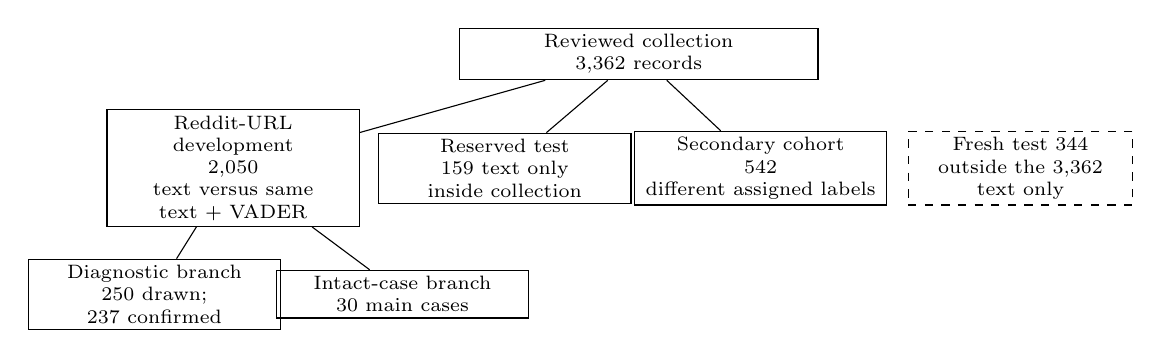
\begin{tikzpicture}[
  font=\scriptsize,
  box/.style={draw, align=center, inner sep=2.2pt, text width=3.05cm},
  freshbox/.style={draw, dashed, align=center, inner sep=2.2pt, text width=2.7cm},
  link/.style={-}
]
\node[box, text width=4.4cm] (col) at (0,0) {Reviewed collection\\3,362 records};
\node[box] (dev) at (-5.15,-1.45) {Reddit-URL development\\2,050\\text versus same text + VADER};
\node[box] (res) at (-1.7,-1.45) {Reserved test\\159 text only\\inside collection};
\node[box] (sec) at (1.55,-1.45) {Secondary cohort\\542\\different assigned labels};
\node[freshbox] (fresh) at (4.85,-1.45) {Fresh test 344\\outside the 3,362\\text only};
\node[box] (diag) at (-6.15,-3.05) {Diagnostic branch\\250 drawn; 237 confirmed};
\node[box] (case) at (-3.0,-3.05) {Intact-case branch\\30 main cases};
\draw[link] (col) -- (dev);
\draw[link] (col) -- (res);
\draw[link] (col) -- (sec);
\draw[link] (dev) -- (diag);
\draw[link] (dev) -- (case);
\end{tikzpicture}
\caption{Separate analyses of the reviewed collection. Lines show which records an analysis uses. The diagnostic sample and the 30 cases are sibling branches under development, not a sequence. Six main cases also occur in the 237; the case list was not drawn from that sample. The fresh test is dashed because it is outside the collection and has no parent link. No line runs from sentiment or purpose scores to reviewer actions.}
\label{fig:design}
\end{figure*}

\begin{table}[t]
\caption{Populations used below. Test scores are text-only.}
\label{tab:pop}
\centering
\footnotesize
\setlength{\tabcolsep}{3pt}
\begin{tabular}{lrrl}
\toprule
Population & Rows & Pos. & Negative class \\
\midrule
Combined collection & 3,362 & --- & Mixed sources \\
Reddit-URL development & 2,050 & 1,658 & 392 other update \\
\quad dissatisfaction type & 68 & 0 & Inside the 392 \\
\quad other type & 324 & 0 & Inside the 392 \\
Non-Reddit URL records & 30 & 28 & Excluded \\
Secondary assigned cohort & 542 & 86 & 456 dissatisfaction \\
Reserved test & 159 & 135 & 24 other update \\
Fresh test & 344 & 277 & 67 other update \\
Diagnostic draw & 250 & --- & Then reconfirmed \\
Diagnostic confirmed & 237 & 237 & Troubleshooting only \\
Intact cases & 30 & --- & Exploratory \\
\bottomrule
\end{tabular}
\end{table}

\section{Methods}
\subsection{Annotation and provenance}
A current-task label requires a reviewed software scope and an update connection. The positive class is troubleshooting. Review provenance for the full collection is mixed: some portions were reviewed with assistance, some were reviewed jointly, and some were held for pilots or protected tests. We therefore do not call the collection an independent gold set, and we do not revise stored labels after test scores were known. The fresh-test labels are a user-reported joint review; the saved freeze record states that no independent first-pass agreement can be estimated from the files. The diagnostic sample is also a joint review record and has no separate field-level agreement statistic. The 30-case record states that two reviewers with software-engineering knowledge completed separate first passes. No field records that a comment resolved a problem. Absence of such a field is an unknown outcome.

The \texttt{releasetrain-sentiment} 0.2.1 package was inspected and not used. Its author average is the mean of stored author comments, or zero when none is stored. The secondary-cohort trajectories can use the post title in that case. Those two constructions are not interchangeable.

\subsection{Purpose classifier and grouped thresholds}
The text model is word and bigram TF--IDF, minimum document frequency 2, at most 20,000 features, and sublinear term frequency, followed by class-balanced logistic regression with $C=4$, the liblinear solver, and random state 42. The vectorizer is fit inside each training fold. Near-duplicate posts stay together: groups are the union of pairs whose normalized title-plus-body character five-gram Jaccard is at least 0.92. Development scores use five-fold stratified group splits with shuffle and seed 42.

For the development comparisons in RQ2, the decision threshold is chosen only on the outer training split. Three inner stratified group folds, also seed 42, score a grid from 0.20 to 0.80 in steps of 0.05. The selected cutoff maximizes mean inner macro-F1, then mean inner F1 of the other-update class, then closeness to 0.5. Outer-fold labels never choose the cutoff. The reserved and fresh tests use one previously fixed specification and the saved continuity threshold 0.588. They were not rescored for this paper, and sentiment features were not attached to them. Fresh majority and fixed-keyword scores come from the same saved test file. The fixed-keyword rule looks for predefined malfunction and recovery cues. It is a text heuristic, not a sentiment model.

\subsection{Sentiment construction}
VADER 3.3.2 supplies the compound score \cite{Hutto2014VADER}. On title and body, the input is the raw title, a newline, and the raw body. An empty or whitespace document returns 0.0, which collides with genuine neutral text. On the 2,050 Reddit-URL posts, 303 bodies are empty and 237 title-body compounds are exactly zero. The primary comparison adds only that one compound to the same title-and-body string. The first comparison is therefore text versus the same text plus one sentiment column. Scalers, like vectorizers, are fit on the training fold only.

A second comparison is limited to the 797 Reddit-URL posts with at least one nonempty stored comment. Both models see one full-thread string: the chosen snapshot title, the body, then nonempty comments in timestamp order. The augmented model adds the title-body compound, the mean of author comments or zero, the mean of community comments or zero, and two missingness flags. An author comment is marked by the stored submitter flag or an author-name match. The title is not used as an author-comment fallback in this comparison. All 7,388 nonempty comments in that subset have timestamps at or after the post, so the features are retrospective. A predeclared bar for a strong comment-feature claim required both an author comment and a community comment on at least half of the 2,050 posts. The observed both-role count is 466 (22.7\%), so comment models stay limited descriptions.

Paired differences are macro-F1 of the augmented model minus macro-F1 of the text model. Intervals use 1,000 bootstrap resamples with seed 42, both by post and by duplicate group. A keyword-first rule that returns troubleshooting whenever technical cues are present is reported only as a heuristic.

Comment storage is uneven (Table~\ref{tab:cov}). On the 2,050 Reddit-URL posts, 797 have a nonempty stored comment: 560 troubleshooting and 237 other-update. Author replies are stored for 362 troubleshooting and 112 other-update posts; community comments for 554 and 235; both roles for 356 and 110. No stored comment remains for 1,098 of 1,658 troubleshooting posts and 155 of 392 other-update posts. The 30 non-Reddit URL records contribute no comments. Coverage is a property of the snapshot, not of the live thread.

\begin{table}[t]
\caption{Stored-comment coverage on 2,050 Reddit-URL posts.}
\label{tab:cov}
\centering
\footnotesize
\setlength{\tabcolsep}{4pt}
\begin{tabular}{lrr}
\toprule
Stored text & Trouble & Other \\
\midrule
Nonempty comment & 560 & 237 \\
Author reply & 362 & 112 \\
Community comment & 554 & 235 \\
Both roles & 356 & 110 \\
No stored comment & 1,098 & 155 \\
\bottomrule
\end{tabular}
\end{table}

\subsection{Diagnostic codebook}
The diagnostic sample is a simple random draw of 250 posts from the then-current 1,658 Reddit-URL troubleshooting development rows, taken before the diagnostic answers. A 50-post feasibility exercise and a 15-post rule check preceded the frozen guide and are not added into the 250. Ten sampled posts overlapped that earlier exercise by chance; their main-study answers were recorded separately under the final guide.

Coders read only the saved title and body. Community name, candidate route, old labels, model scores, comments, and live pages were out of scope. The first decision reconfirmed troubleshooting: yes, no, or unclear. Field summaries are conditional on yes. Eight fields were then marked present, not observed, or unclear: software product, identifiable release, environment, specific symptom, reproduction context, error evidence, attempted remedy, and an explicit help request. An identifiable release needs a version, build, named release, or unambiguous cycle; ``latest update'' alone is not enough. Reproduction context needs an action or condition, not timing alone. Error evidence needs a specific message, code, log, trace, or described diagnostic output. An image that is referenced but unreadable can make that field unclear. A remedy must have been attempted. Not observed means not visible in the snapshot. It is not proof that the fact was absent from the incident. No overall usefulness score was assigned. The 13 posts marked no or unclear stay in the classifier snapshot; diagnostic exclusion does not relabel them. Table~\ref{tab:code} records the present-rule used for each field. The same guide states that a blank body does not automatically make every field unclear.

\begin{table}[t]
\caption{Present-rule for the eight diagnostic fields. Not observed means not visible in the saved title or body.}
\label{tab:code}
\centering
\footnotesize
\setlength{\tabcolsep}{3pt}
\begin{tabular}{lp{4.6cm}}
\toprule
Field & Counted present when the text gives \\
\midrule
Product & An app, OS, service, tool, or component \\
Release & A version, build, named release, or unique cycle \\
Environment & A device, OS, host, or configuration \\
Symptom & Concrete wrong behavior \\
Reproduction & An action or condition for that behavior \\
Error evidence & A message, code, log, trace, or described output \\
Remedy & A fix or workaround actually tried \\
Help request & An explicit request for diagnosis or a fix \\
\bottomrule
\end{tabular}
\end{table}

\subsection{Thirty intact cases}
After a six-post pilot, excluded from the counts, two reviewers read 30 purposefully selected intact title-and-body snapshots. The cases were varied by community, update situation, symptom, evidence, and expected difficulty. Each reviewer chose one first action: open an update-focused investigation, request a specific clarification, monitor or group similar reports, take no update-focused action, or mark the case unassessable. They also named the evidence they used. The assigned discussion label was hidden. Counts describe these 30 cases and these two readers only. They were not crossed with VADER scores, and they are not a population rate. Saved identifiers show that the 30 are not a subset of the 237: six main-case rows also appear in the confirmed diagnostic sample, and the case list was not drawn from that sample. The six pilot cases are excluded from the counts.

\section{Results}
\subsection{Purpose detection}
Table~\ref{tab:purpose} reports the saved text-only tests. Fresh macro-F1 is 0.792, above the fresh majority score of 0.446 and the fixed-keyword score of 0.474. The fresh confusion matrix is 46 of 67 other-update posts and 252 of 277 troubleshooting posts correct. Other-update F1 on that test is 0.667. The reserved score is 0.863, with 18 of 24 other-update posts and 130 of 135 troubleshooting posts correct, and other-update F1 0.766. The two tests use the same specification and different fitted training populations, so the drop is descriptive rather than a controlled transfer estimate. Framing these evaluations with the later sentiment and case analyses does not raise either score.

On the 2,050-post development text, the same grouped protocol gives logistic regression macro-F1 0.832. A linear SVM with the same TF--IDF and its default margin scores 0.820. A keyword-first heuristic scores 0.685. Multinomial naive Bayes, which is not class-balanced in this run, scores 0.551 and predicts every troubleshooting post as troubleshooting (confusion 43 and 349 on the other-update class, and 0 and 1,658 on troubleshooting). These are text baselines. They are not evidence that a sentiment feature helps.

\begin{table}[t]
\caption{Text-only purpose scores. No sentiment feature is included.}
\label{tab:purpose}
\centering
\footnotesize
\begin{tabular}{lrl}
\toprule
Evaluation & $n$ & Macro-F1 \\
\midrule
Reserved test & 159 & 0.863 \\
Fresh test & 344 & 0.792 \\
Fresh majority & 344 & 0.446 \\
Fresh fixed keyword & 344 & 0.474 \\
\bottomrule
\end{tabular}
\end{table}

\subsection{Where valence separates, and where it does not}
On all 2,050 Reddit-URL posts, text macro-F1 is 0.832 and the same text plus the title-body compound is 0.833 (Table~\ref{tab:sent}). The difference is $+0.001$. The post-level 95\% interval is $-0.012$ to $+0.015$, and the duplicate-group interval is $-0.013$ to $+0.015$. Both include zero. Other-update F1 changes by $+0.001$, and that interval also includes zero. VADER alone scores 0.534, near the majority baseline of 0.447. The classifier is using lexical purpose cues. The compound does not add a reliable increment on this task.

Figure~\ref{fig:valence} shows why a class-mean plot can still look informative. Mean title-body compound is $-0.064$ for troubleshooting ($n=1{,}658$) and $+0.194$ for the pooled other-update class ($n=392$). Splitting that negative class, the 324 posts of type \texttt{other} have mean $+0.249$, while the 68 dissatisfaction posts have mean $-0.068$. The troubleshooting-versus-dissatisfaction difference is $+0.004$, and its interval includes zero. Text classification of that 1,726-post pair reaches macro-F1 0.658 because the classes are highly unbalanced; adding the compound changes it by $+0.010$, and that interval includes zero. VADER alone predicts every one of those 1,726 posts as troubleshooting. The average gap against ``other update discussion'' is therefore not a gap against confirmed dissatisfaction. Much of the positive mass sits in update talk that was not labeled as dissatisfaction.

A closed-list description on the same 2,050 posts points the same way and is not a causal mask. Incident terms appear in 1,258 of 1,658 troubleshooting posts (76\%) and in 154 of 392 other-update posts (39\%). Discontent terms appear in about 10\% and 11\% of those classes. Posts with discontent terms and no incident terms are few: 33 troubleshooting posts, mean compound $-0.275$, and 13 other-update posts, mean $-0.223$. Technical wording and evaluative wording are not the same partition as the purpose label.

\begin{table}[t]
\caption{Development macro-F1. Augmented models add sentiment columns to the same text.}
\label{tab:sent}
\centering
\footnotesize
\setlength{\tabcolsep}{3pt}
\begin{tabular}{lrrr}
\toprule
Comparison & Text & Plus sent. & Diff. \\
\midrule
Title/body, $n{=}2{,}050$ & 0.832 & 0.833 & $+0.001$ \\
Dissatisfaction pair, $1{,}726$ & 0.658 & 0.668 & $+0.010$ \\
Full thread, $n{=}797$ & 0.866 & 0.839 & $-0.027$ \\
\bottomrule
\end{tabular}
\end{table}

\begin{figure}[t]
\centering
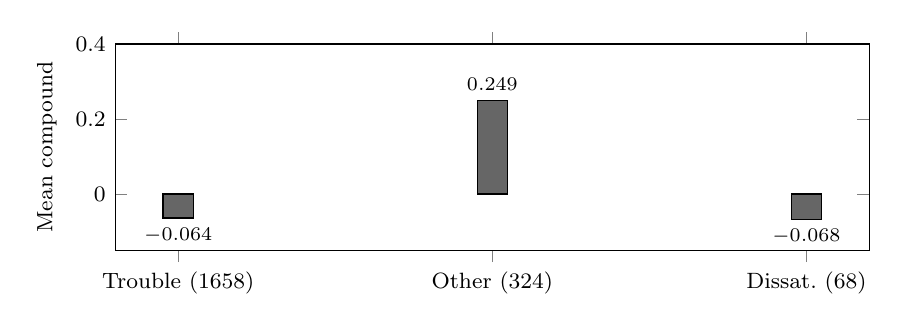
\begin{tikzpicture}
\begin{axis}[
    ybar,
    width=0.92\columnwidth,
    height=4.2cm,
    ymin=-0.15, ymax=0.40,
    ylabel={Mean compound},
    ylabel style={font=\footnotesize},
    symbolic x coords={T,O,D},
    xtick=data,
    xticklabels={Trouble (1658),Other (324),Dissat.\ (68)},
    x tick label style={font=\footnotesize},
    y tick label style={font=\footnotesize},
    bar width=11pt,
    nodes near coords,
    every node near coord/.append style={font=\scriptsize, /pgf/number format/fixed, /pgf/number format/precision=3},
]
\addplot[fill=black!60] coordinates {(T,-0.064) (O,0.249) (D,-0.068)};
\end{axis}
\end{tikzpicture}
\caption{Mean title-body VADER compound on the 2,050 Reddit-URL development posts, split by assigned discussion type. Trouble and Dissat.\ are close. The positive mean is the other discussion type inside the current negative class. The panel is descriptive, not a causal contrast.}
\label{fig:valence}
\end{figure}

Among 797 posts with a stored comment, full-thread text scores 0.866 and the same text plus sentiment columns scores 0.839. The difference is $-0.027$. Post-level and group-level intervals both exclude zero on this subset (group interval $-0.051$ to $-0.005$). Only 14 of the 797 posts share a duplicate group, so that exclusion is a weak dependence correction, not a general claim that sentiment features harm classification. Stored comments are missing for 1,098 of 1,658 troubleshooting posts (66\%) and for 155 of 392 other-update posts (40\%). All 30 non-Reddit URL records lack a stored comment. The lower thread score is a selected, retrospective result.

The secondary cohort has 86 posts assigned as technical problem statements and 456 assigned as general dissatisfaction. Full-file author--community divergence is 0.371 versus 0.287 (Mann--Whitney $p=0.009$). Author means are 0.009 versus 0.191; community means are 0.168 versus 0.194 (Welch $p=0.33$). Author tracks use the title alone for 205 posts. After those tracks are removed, author means remain lower for the technical class (0.077 versus 0.261), but divergence is no longer distinguished at $p=0.05$ ($p=0.060$). Author slope is not significant. This cohort uses a different label system from the 2,050-post task, including the 68-post dissatisfaction slice of that task.

\subsection{Diagnostic visibility}
Reconfirmation of the 250-post draw kept 237 troubleshooting posts, marked four as not troubleshooting, and left nine unclear. Table~\ref{tab:fields} and Figure~\ref{fig:fields} use the signed conditional counts on those 237. A specific symptom is recorded for every retained post, which partly follows from reconfirming the troubleshooting designation. Error evidence is present in 40 posts (16.9\%; Wilson 12.6--22.2\%). Seven further error-evidence decisions were unclear and are not counted as absence. Reproduction context is present in 108 (45.6\%). The mean number of present fields is 4.84 of eight, an unweighted description rather than a utility score.

The 20 posts without a saved body are the confirmed subset of a larger fact: 24 of the 250 sampled posts had no saved body, and 20 of those 24 were confirmed troubleshooting (\texttt{title\_only} $n=20$ in the signed body split; 217 had a body). Reproduction context is present in 2 of those 20 and in 106 of the 217. An attempted remedy is present in 2 of 20 and in 116 of 217. An exploratory join to grouped development predictions, whose macro-F1 on that development run is 0.835, found 16 misses among the 237, including 8 of the 20 title-only posts and 8 of the 217 with a body. That join is descriptive. It does not show that a missing body caused a miss, and the diagnostic fields were not coded on the fresh test.

\begin{table}[t]
\caption{Fields present in the saved title or body of 237 reconfirmed troubleshooting posts.}
\label{tab:fields}
\centering
\footnotesize
\setlength{\tabcolsep}{3pt}
\begin{tabular}{lrrr}
\toprule
Field & Present & \% & Wilson \\
\midrule
Software product & 218 & 92.0 & 87.8--94.8 \\
Identifiable release & 122 & 51.5 & 45.1--57.8 \\
Environment & 137 & 57.8 & 51.4--63.9 \\
Specific symptom & 237 & 100 & 98.4--100 \\
Reproduction context & 108 & 45.6 & 39.4--51.9 \\
Error evidence & 40 & 16.9 & 12.6--22.2 \\
Attempted remedy & 118 & 49.8 & 43.5--56.1 \\
Help request & 168 & 70.9 & 64.8--76.3 \\
\bottomrule
\end{tabular}
\end{table}

\begin{figure}[t]
\centering
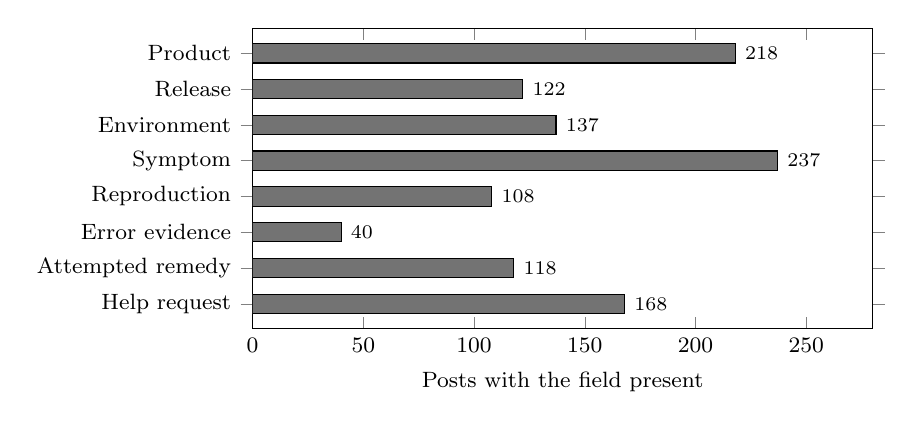
\begin{tikzpicture}
\begin{axis}[
    xbar,
    width=0.78\columnwidth,
    height=5.4cm,
    xmin=0, xmax=280,
    xlabel={Posts with the field present},
    symbolic y coords={Help,Remedy,Error,Repro,Symptom,Environ.,Release,Product},
    ytick=data,
    yticklabels={Help request,Attempted remedy,Error evidence,Reproduction,Symptom,Environment,Release,Product},
    y tick label style={font=\footnotesize},
    x tick label style={font=\footnotesize},
    xlabel style={font=\footnotesize},
    nodes near coords={\pgfmathprintnumber{\pgfplotspointmeta}},
    every node near coord/.append style={font=\scriptsize, /pgf/number format/fixed},
    bar width=7pt,
]
\addplot[fill=black!55] coordinates {(168,Help) (118,Remedy) (40,Error) (108,Repro) (237,Symptom) (137,Environ.) (122,Release) (218,Product)};
\end{axis}
\end{tikzpicture}
\caption{Present counts from Table~\ref{tab:fields}. The symptom count follows reconfirmation. Seven unclear error-evidence decisions are omitted rather than treated as absence.}
\label{fig:fields}
\end{figure}

\subsection{Purpose is not the first action}
The two reviewers chose the same first action in 21 of the 30 cases and different actions in nine. Both chose investigation in ten cases, clarification in six, monitoring in one, and no update-focused action in four. One reader selected investigation 16 times and the other 11 times; the second selected monitoring five times and the first once. In the nine disagreements, the written explanations often cited overlapping facts and differed on whether those facts were sufficient to act, which question should come first, or whether wider impact was established. One post assigned to other update discussion led both readers to investigate. A reported workaround did not map to one action across cases. These contrasts show that a purpose label is not an action key. The written explanations add three boundary patterns, stated here without post identifiers. Concrete update-linked failures, together with a comparison or a recovery impact, could support investigation in some of these cases. A concrete symptom did not always settle the next action: in one browser-crash case both reviewers wanted a normal-versus-private-window comparison first, and in one storage case both wanted the space measurement clarified. A reported workaround did not map to one action. Both reviewers opened a lead for one editor case that already had a workaround, whereas in two other cases one reviewer opened a lead and the other preferred monitoring. Some dissatisfaction-labeled posts described concrete changed behavior and still led to different actions.

\section{Discussion}
Three separations follow from the results, and none of them is a pipeline.

First, the valence gap is a property of the negative class that is used. Against the broad other-update class, troubleshooting text is more negative on average. Against the 68 posts confirmed as dissatisfaction, that average gap is gone, and adding the compound does not reliably change classification. A plot that pools advice, reactions, and dissatisfaction into one negative class will attribute to ``sentiment versus troubleshooting'' a difference that is largely ``other discussion versus troubleshooting.'' The secondary cohort, whose negative class is assigned dissatisfaction, can still show an author-track difference. That result belongs to its own labels. It does not restore the gap on the 68-post slice, and it does not license pooling the 542 with the 2,050.

Second, the purpose classifier and the sentiment score are not substitutes. Title and body text beats majority and fixed-keyword baselines on the fresh test, including a lower other-update F1 of 0.667 that should stay visible next to the headline 0.792. VADER alone is close to the majority baseline. Adding it to the same development text leaves an interval that includes zero. Adding sentiment columns to a full thread, on the minority of posts that have comments, lowers macro-F1 in this sample. That lower score is reported because it is what the comparison produced. It is not evidence that sentiment is generally harmful, and it is not evidence that a comment fixed an issue. The practical reading is narrower: for this purpose task, the useful signal in the saved text is not well summarized by a compound score.

Third, detecting troubleshooting does not decide what an engineer should do next. In the 237 confirmed posts, a product name is usually visible and a specific symptom was required by reconfirmation, but error evidence and reproduction context are often not in the snapshot. Twenty confirmed posts have no body at all, and those 20 account for half of the 16 development misses in the exploratory join. In the 30 intact cases, reviewers sometimes chose different first actions from overlapping facts, and one post outside the troubleshooting class still drew investigation from both. Purpose classification can organize a queue. It does not certify that the snapshot is sufficient, and it does not replace the judgment the two reviewers recorded.

\section{Threats}
The collection comes from candidate routes plus assigned labels, not a random sample of Reddit. Thirty records have non-Reddit URL metadata and are excluded from the primary results. The fresh and reserved scores belong to separate fits of the same specification. Comment missingness differs by class, and both-role coverage is below the predeclared bar. VADER returns zero for an empty document. The technical-word lists were fixed before counting and exclude the words ``update'' and ``upgrade'' because the collection is update-scoped; they are not a masking experiment. Diagnostic coding has one joint review record. The 30 cases were purposefully varied. No causal effect of sentiment, fields, or the classifier on engineering work is identified.

\section{Conclusion}
Reddit software-update posts support three limited descriptions. Title and body text separate troubleshooting from other update discussion on held-out Reddit-URL posts, with fresh macro-F1 0.792 and reserved macro-F1 0.863, both text-only. A VADER compound does not reliably add information to the same development text, and the dissatisfaction subset does not reproduce the valence gap seen against other update discussion. Saved troubleshooting text often lacks error evidence, reproduction context, or a body. Two reviewers, reading 30 intact posts, sometimes chose different first actions from similar facts. Each result stays within its sample. None of them raises the others, and together they are not an evaluated triage pipeline.

\section*{Acknowledgment}
OpenAI Codex assisted with scientific planning, source audit, outline and review comments, and literature checking. Cursor assisted with substantive drafting and organization of the abstract, introduction, related work, methods, results, discussion, threats, and conclusion, and with the LaTeX, tables, and figures drawn from saved counts. The authors are responsible for verifying the claims, citations, and final wording. Neither tool created the human review labels, diagnostic codes, or the reviewers' first-pass actions. The disclosure follows the IEEE author guidelines for AI-generated text \cite{IEEE2024AIText}.

\bibliographystyle{IEEEtran}
\bibliography{references}
\end{document}
